In order to support priorities and static/moving nodes, the work queue of each
thread presented in Fig.~\ref{fig:implementation:vm_overview} must be extended.
For that, we updated the queue implementation to include two pairs of queues:
a pair of doubly linked lists known as the \emph{standard queue} and a pair of
\emph{min/max} heaps known as the \emph{priority queue}.  The standard queue
contains nodes without priorities and supports push into tail, remove node from
the head, remove arbitrary node, and remove first half of nodes.  The priority
queue contains nodes with priorities and is implemented as a binary heap array.
It supports the following operations: push into the heap, remove the \emph{min}
node, remove an arbitrary node, remove half of the nodes (horizontal split), and
priority update.  Operations for removing half of the queue are implemented in
order to support node stealing, while operations to remove arbitrary nodes or
update priority allows threads to change the priority of nodes.
Table~\ref{fig:implementation:table_queue} show the complexity of queue
operations and compares the standard queue against the priority queue.

\begin{table}[h]
   \begin{tabular}{| c | l | l |}
      \hline
      \textbf{Operation} & \textbf{Standard queue} & \textbf{Priority Queue} \\
      \hline
      Push & $\mathcal{O}(1)$ & $\mathcal{O}(\log{N})$ \\ \hline
      Pop & $\mathcal{O}(1)$ & $\mathcal{O}(\log{N})$ \\ \hline
      Remove & $\mathcal{O}(1)$ & $\mathcal{O}(\log{N})$ \\ \hline
      Remove Half & $\mathcal{O}(N)$ & $\mathcal{O}(\log{N})$ \\ \hline
      Priority Update & - & $\mathcal{O}(\log{N})$ \\ \hline
   \end{tabular}
   \caption{Comparing the complexity of queue operations for both standard
      queue and priority queue. Except for the remove half operation, priority
      queue operations are more expensive.}
   \label{fig:implementation:table_queue}
\end{table}

\begin{figure*}[t]
\centering
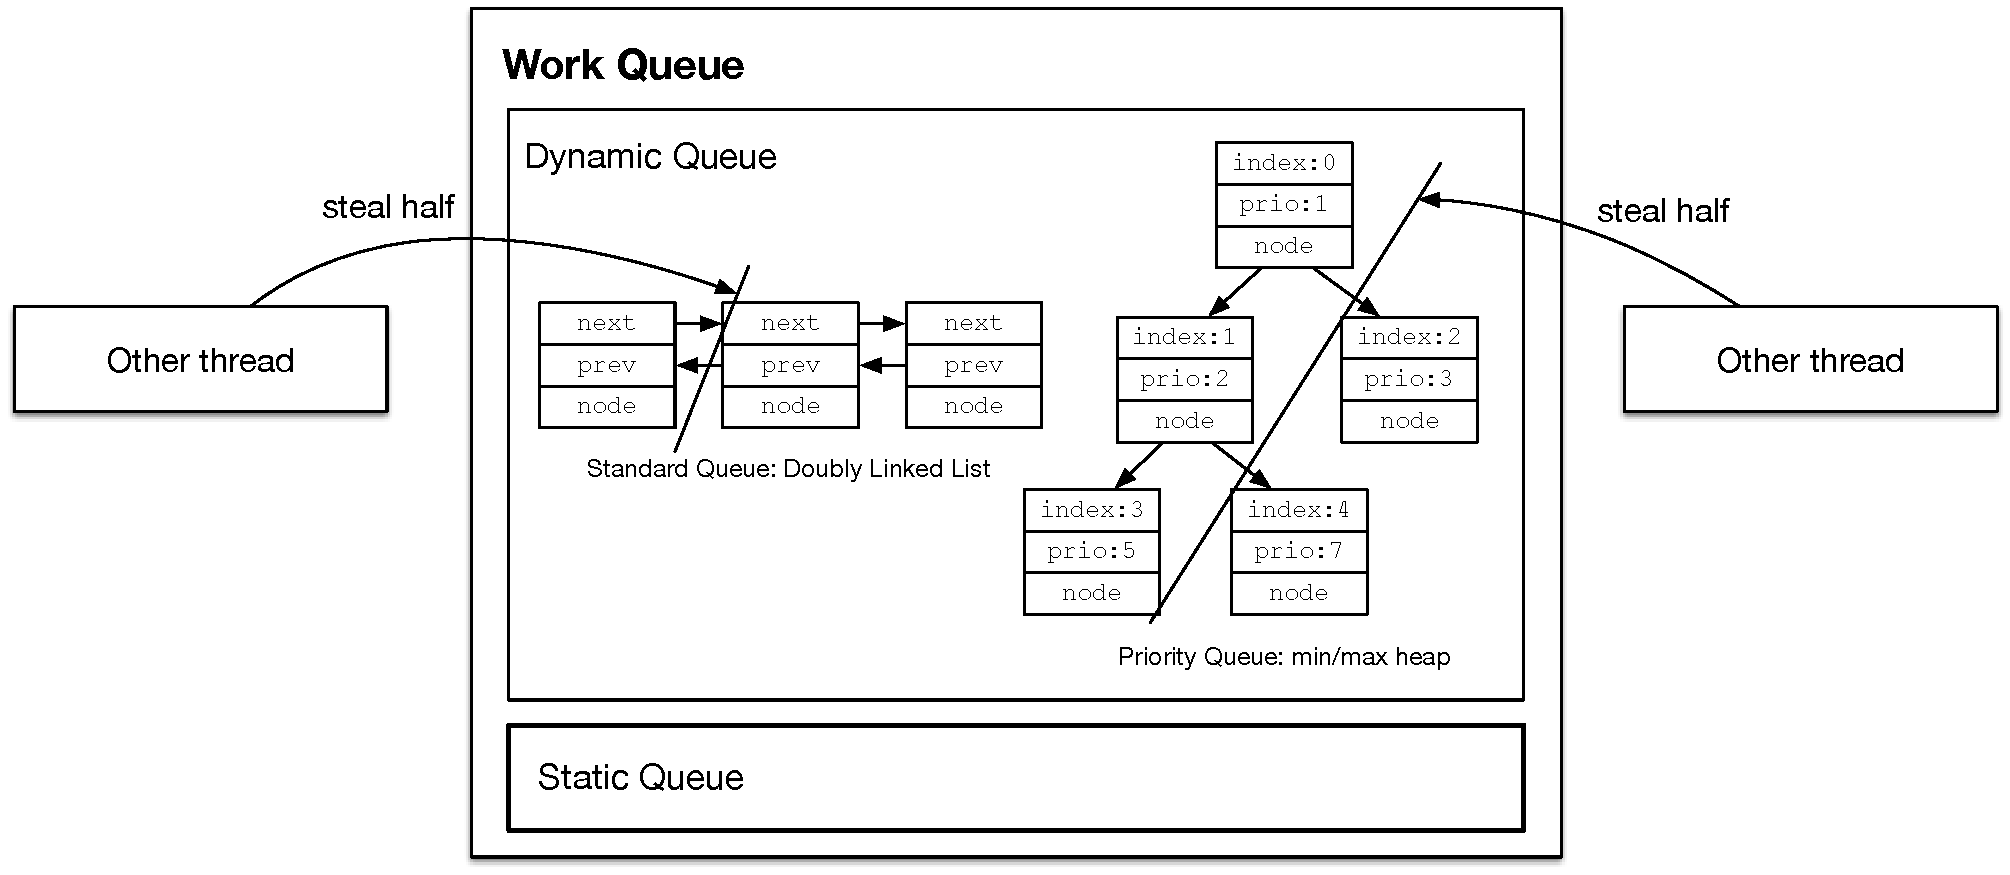
\includegraphics[width=0.95\textwidth]{figures/implementation/work_queue.pdf}
\caption{Thread's work queue and its interaction with other threads: the dynamic queue contains nodes that can be
   stolen while the static queue contains nodes that cannot be stolen. Both
   queues are implemented with one standard queue and one priority queue.}
\label{fig:implementation:work_queue}
\end{figure*}

The \texttt{next} and \texttt{prev} pointers of the regular queue are part of
the node structure in order to save space. These pointers are also used as the
index in the priority queue and current priority, respectively. Both the regular
and priority queue are implemented as a pair of queues.  This first queue is the
\emph{static queue} which contains nodes that cannot be stolen.  The other queue
is the \emph{dynamic queue} which contains nodes which can be stolen by other
threads.

To minimize inter-thread communication, node priorities are implemented at the
thread level. Thus, when a thread picks the highest priority node from the
priority queue, it is only the highest priority with respect to the set of nodes
owned by the thread and not the highest priority node in the whole program.  

\subsection{Node State Machine}\label{sec:node_state_machine}

We added a new node state to the state machine presented in
Fig.~\ref{fig:local:node_states} to accommodate the new coordination facilities.
We review the states of the state machine presented in
Fig.~\ref{fig:implementation:node_states}:

\begin{itemize}
   \item \textbf{running}: the node is deriving rules.
   \item \textbf{inactive}: the node is inactive, i.e., it has no new facts and is not in any
   queue for processing.
   \item \textbf{active}: the node has new facts and is in some queue waiting
   to be processed.
   \item \textbf{stealing}: the node has just been stolen and is in the process of being
   moved to another thread.
   \item \textbf{coordinating}: the node is moving from one queue to another.
\end{itemize}

\begin{figure}[ht]
   \centering
   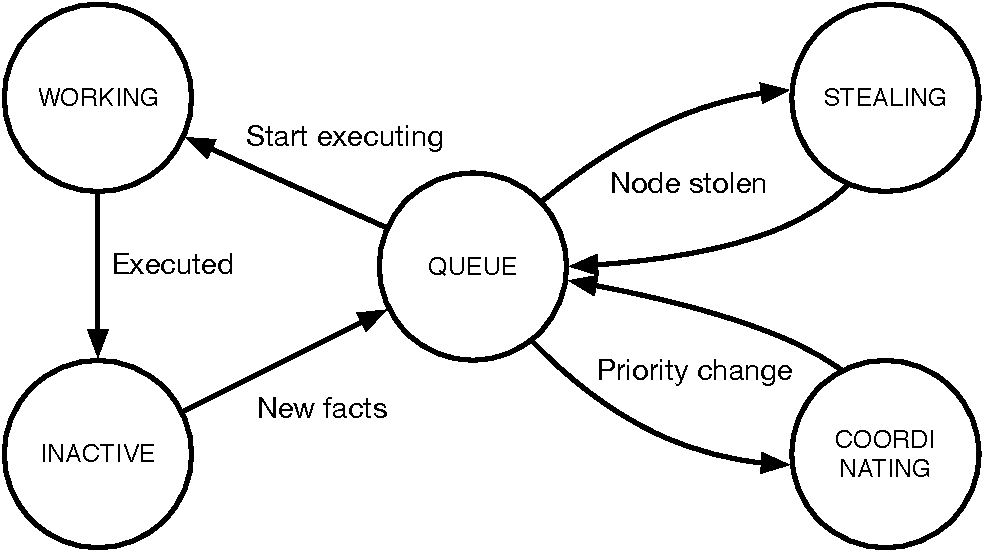
\includegraphics[width=0.55\textwidth]{figures/implementation/node_states.pdf}
   \caption{The node state machine as represented by the state variable. During
      the lifetime of a program, each node goes through different states as
      specified by the state machine.}
   \label{fig:implementation:node_states}
\end{figure}

\subsection{Communication And Locks}

When a thread $T_1$ needs to perform coordination operations to a node in thread
$T_2$ then it needs to synchronize with $T_2$. The target node lock always needs
to be acquired.  Optionally, we may need to also lock the queues of the current
thread $T_1$ or $T_2$.  Note that both the standard queue and priority
queue have separate locks in order to allow concurrent manipulation of the two
data structures.
